\documentclass{article}

\usepackage{graphicx}
\usepackage{tikz}
\usepackage{tikzsymbols}
\usetikzlibrary{calc,patterns,shapes.geometric}
\pagestyle{empty}
\usepackage[margin=0pt]{geometry}
\geometry{papersize={14in,12in}}

\def\centerarc[#1](#2)(#3:#4:#5){\draw[#1] ($(#2)+({#5*cos(#3)},{#5*sin(#3)})$) arc (#3:#4:#5);}

\begin{document}
	\begin{figure}
		\centering
		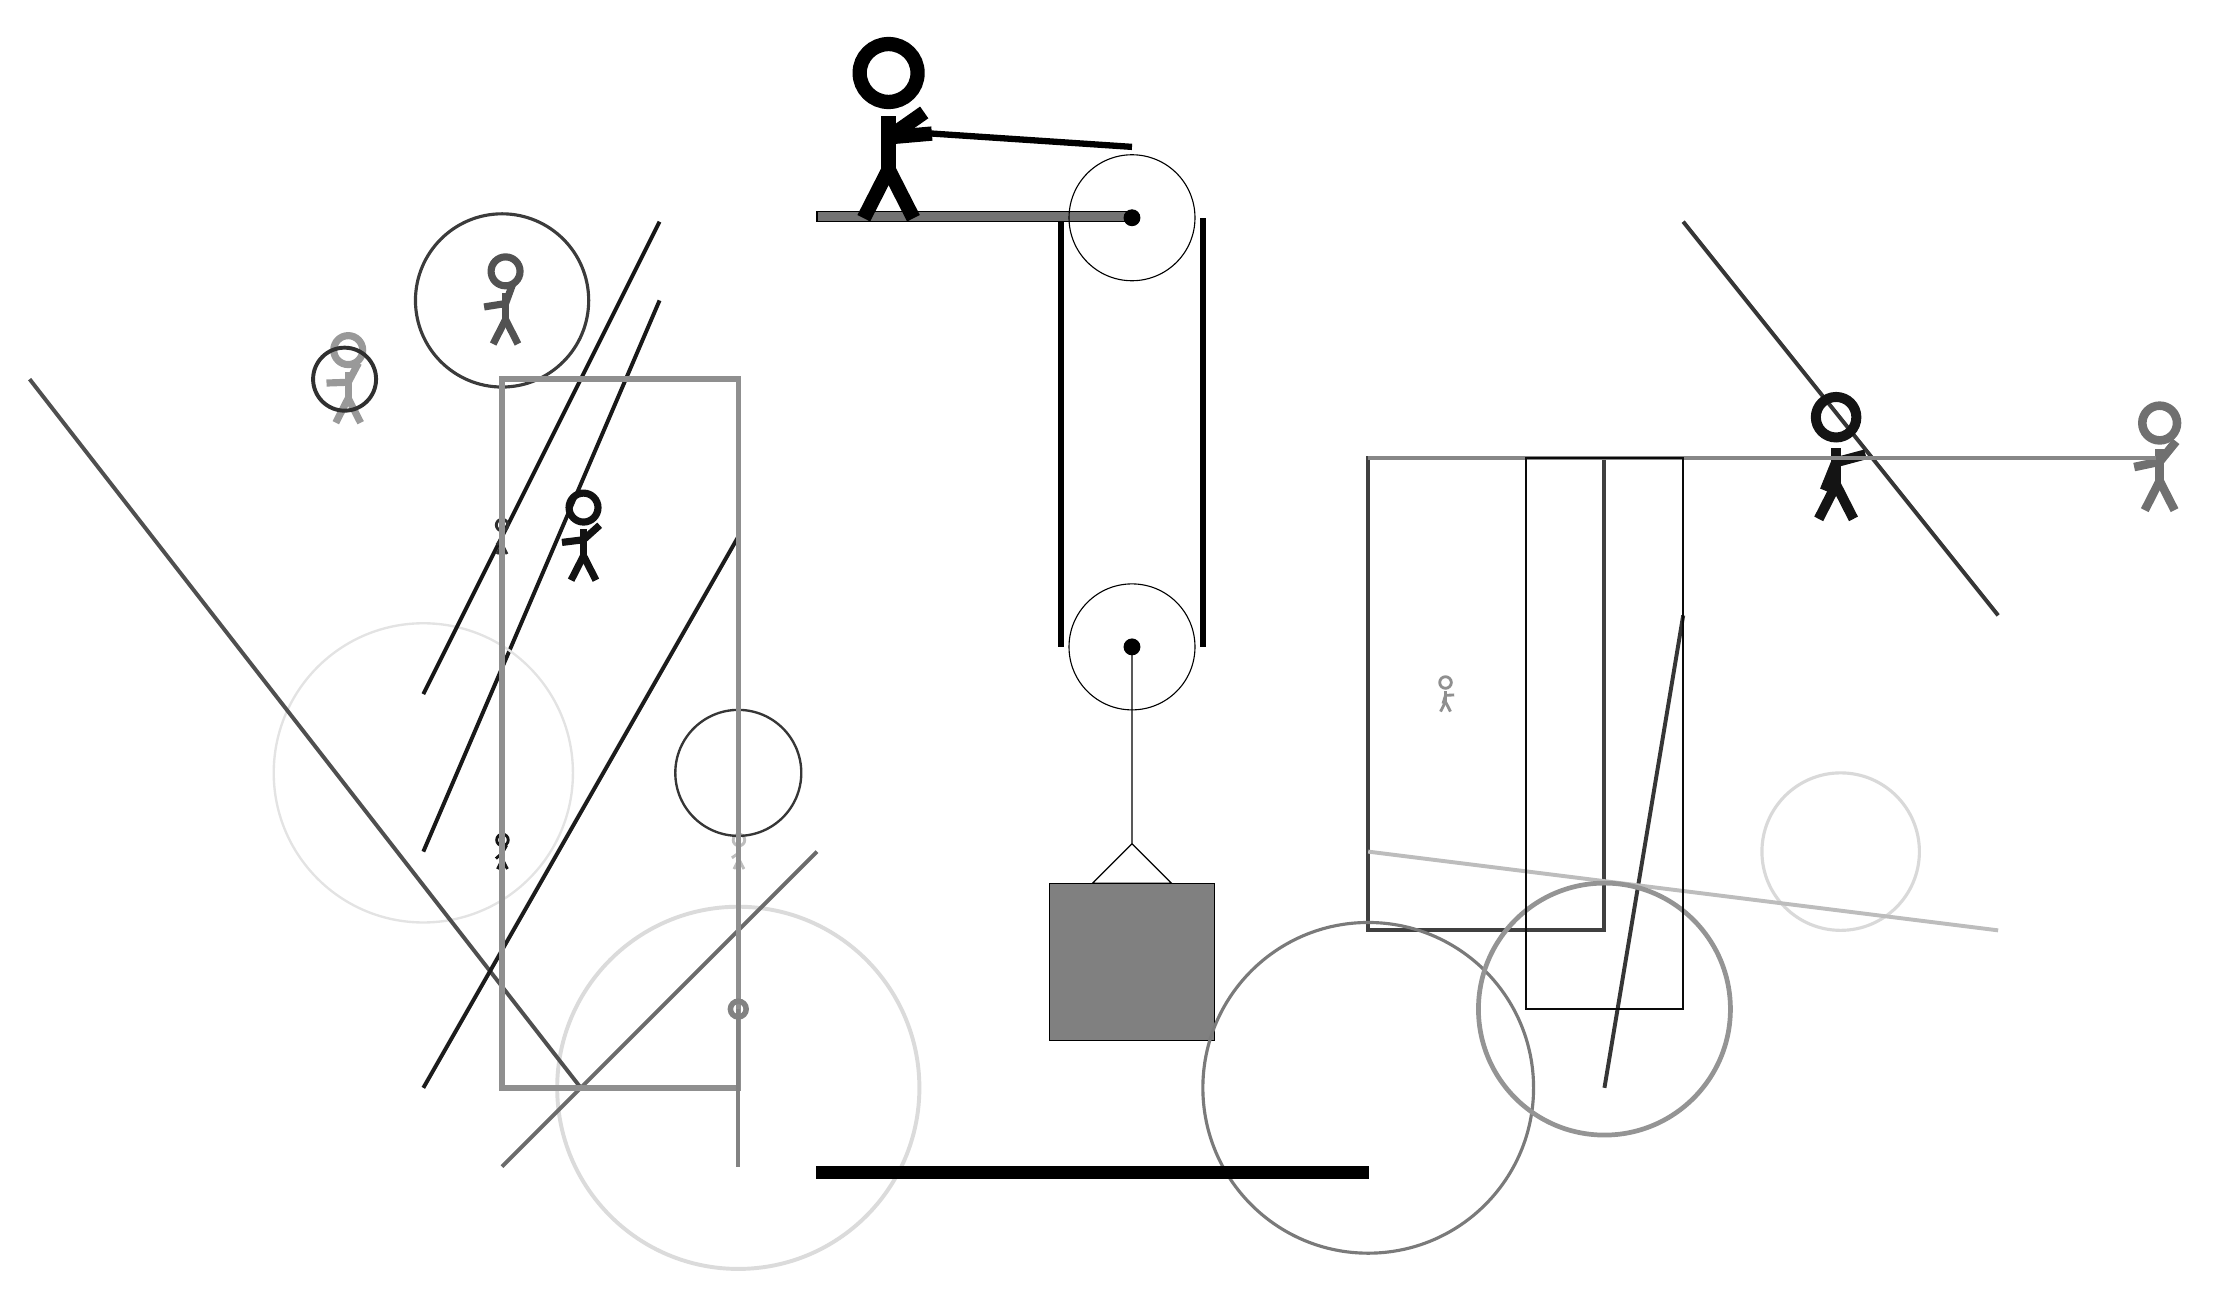
\begin{tikzpicture}
			%%%%% START %%%%%
			
			\draw[fill=black!55] (-2, 9) rectangle (2, 9.125);
			
			\draw (2, 3.6) circle (0.8);
			\draw[fill=black] (2, 3.6) circle (0.1);
			
			\draw (2, 9.05) circle (0.8);
			\draw[fill=black] (2, 9.05) circle (0.1);
			
			\draw (2, 3.6) -- (2, 1.1) -- (1.5, 0.6) -- (2.5, 0.6) -- (2, 1.1);
			\draw[fill=black!50] (0.95, 0.6) rectangle (3.05, -1.4);
			
			\draw[line width=0.8mm] (1.1, 9) -- (1.1, 3.6);
			\centerarc[line width=0.8mm](2, 3.6)(180:360:0.9);
			\draw[line width=0.8mm](2.9, 3.6) -- (2.9, 9.05);
			\centerarc[line width=0.8mm](2, 9.05)(0:90:0.9);
			\draw[line width=0.8mm](2, 9.95) -- (-1, 10.15);
			
			\node[line width=0.2mm, color=black!40] at (-8, 7) {\Strichmaxerl[5][2][62]};
			
			\draw [line width=0.5mm, color=black!14](-3, -2) circle (2.3);
			\draw[line width=0.5mm, color=black!90](-4, 8) -- (-7, 1);
			\node[line width=0.7mm, color=black!93] at (-5, 5) {\Strichmaxerl[5][7][42]};
			\node[line width=0.5mm, color=black!56] at (15, 6) {\Strichmaxerl[6][12][51]};
			
			\draw [line width=0.5mm, color=black!81](-8, 7) circle (0.4);
			\node[line width=0.5mm, color=black!26] at (-3, 1) {\Strichmaxerl[2][35][84]};
			
			\draw[line width=0.5mm, color=black!75] (5, 0) rectangle (8, 6);
			\node[line width=0.2mm, color=black!44] at (6, 3) {\Strichmaxerl[2][73][3]};
			\draw [line width=0.3mm, color=black!11](-7, 2) circle (1.9);
			
			\node[line width=0.6mm, color=black!68] at (-6, 8) {\Strichmaxerl[5][9][70]};
			
			\draw[line width=0.5mm, color=black!91](-7, 3) -- (-4, 9);
			\node[line width=0.6mm, color=black!82] at (-6, 5) {\Strichmaxerl[2][53][86]};
			
			\draw[line width=0.5mm, color=black!79](9, 9) -- (13, 4);
			\draw[line width=0.5mm, color=black!58](-6, -3) -- (-2, 1);
			\draw [line width=0.4mm, color=black!52](5, -2) circle (2.1);
			
			\node[line width=0.5mm, color=black!92] at (11, 6) {\Strichmaxerl[7][68][15]};
			
			\draw[line width=0.5mm, color=black!69](-5, -2) -- (-12, 7);
			\draw[line width=0.5mm, color=black!47](5, 6) -- (15, 6);
			\draw [line width=0.3mm, color=black!79](-3, 2) circle (0.8);
			\draw [line width=0.4mm, color=black!77](-6, 8) circle (1.1);
			
			\draw[line width=0.5mm, color=black!79](8, -2) -- (9, 4);
			\draw [line width=0.4mm, color=black!15](11, 1) circle (1.0);
			\draw[line width=0.3mm, color=black!88] (7, 2) rectangle (7, 1);
			\draw[line width=0.5mm, color=black!26](5, 1) -- (13, 0);
			
			\draw[line width=0.5mm, color=black!89](-7, -2) -- (-3, 5);
			\draw [line width=0.6mm, color=black!42](8, -1) circle (1.6);
			\node[line width=0.7mm, color=black!92] at (-6, 1) {\Strichmaxerl[2][41][61]};
			\draw[line width=0.7mm, color=black!44] (-3, -2) rectangle (-6, 7);
			\draw[line width=0.2mm, color=black!96] (7, 6) rectangle (9, -1);
			\draw[line width=0.5mm, color=black!49](-3, -3) -- (-3, -1);
			\draw [line width=0.7mm, color=black!49](-3, -1) circle (0.1);
			
			\node at (-1, 10.15) {\Strichmaxerl[10][-175][35]};
			
			\draw[fill=black] (-2, -3) rectangle (5, -3.15);
			
			%%%%% END %%%%%
		\end{tikzpicture}
	\end{figure}	
\end{document}